\documentclass[10pt,pdftex]{report}
\usepackage[T1]{fontenc}
\usepackage[utf8]{inputenc}
\usepackage[magyar]{babel}
\usepackage{graphicx}
\usepackage{amsmath}
\usepackage{amssymb}
\usepackage{multirow}
\usepackage{booktabs}
\usepackage{indentfirst}
\usepackage[a4paper]{geometry}
\usepackage{url}
\usepackage{titling}
\usepackage{float}
\usepackage{spverbatim}
\usepackage{xcolor}
\usepackage{hyperref}
\usepackage{adjustbox}
    \definecolor{titlebg}{RGB}{128,128,128}

\usepackage{lmodern}
\usepackage{etoolbox}
\patchcmd{\thebibliography}{\chapter*}{\section*}{}{}

\renewcommand{\thesection}{\arabic{section}}


\title{Forgómozgás vizsgálata}

%% EZ ALÁBBI KÉT MEZŐT ÉRTELEMSZERŰEN KI KELL TÖLTENI
\author{Bíró Gergő Tamás}
\date{2025. március 25.}


%% FEJLÉC LEÍRÓ, NEM KELL MÓDOSÍTANI
\renewcommand*{\maketitle}{\noindent{%
\parbox{\dimexpr\linewidth-2\fboxsep}{\color{black}%
\parbox{\linewidth}{\fontsize{18}{24}\selectfont\sffamily\bfseries\thetitle}%
}}\vskip 1em%
\begin{tabular}{l}%
Mérést végezte: \theauthor \\%
Mérés dátuma: \thedate\\
Jegyzőkönyv végleges változata: \today \\%
Jegyzőkönyv leadásának időpontja: 2025. április 1.
\end{tabular}%
}
%%%%%%%%%%%%%%%%%%%%%

\begin{document}
\maketitle
\section*{Mérés célja}
A mérés során egy korong és egy rúd tehetetlenségi nyomatékát szeretnénk megmérni, valamint kiszámolni azok fizikai paramétereiből, a tehetetlenségi nyomaték kiszámítására a lkalmazott képlet a korong esetén  $\Theta=\frac{1}{2}mr^2$ a rúdnál pedig $\Theta=\frac{1}{12}mL^2+\frac{1}{4}m\rho^2$ amikben $m$ az adott test tömege, $\Theta$ a test tehetetlenségi nyomatéka, $r$ a korong sugara, $L$ a rúd hossza és $\rho$ pedig a rúd sugara. A két különböző módszerből kapott eredményeket pedig összehasonlítjuk, ezzel megpróbáljuk igazolni a fenti képleteket.
\section*{Mérőeszközök}
\begin{itemize}
    \item{Fonál}
    \item{Fonáltárcsa}
    \item{Súlyok}
    \item{Korong}
    \item{Rúd}
    \item{Vonalzó}
    \item{Mérleg}
    \item{Tolómérő}
    \item{Fénykapus sebességmérő és az ehhez kompatibilis küllőzött csiga}
\end{itemize}
\section*{A mérés leírása}
A mérés során először a korong és a rúd tömegét mérjük meg mérleg segítségével, ezen kívül még a referencia fonáltárcsa tömegét is megmérjük. Ezek után a korong átmérőjét és a henger hosszát vonalzóval, valamint a rúd átmérőjét és az egyes testekhez tartozó fonáltárcsák belső átmérőjét mérjük tolómérő segítségével. A testek paramétereinek meghatározása után az egyik testet befogatjuk, a fonalat átvezetjük a csigán, ezután a súlyt felakaszjuk a fonálra, és a fonalat egy rétegben feltekerjük a fonáltárcsára. Miután ezt megtettük a testet elngedjük, és hagyjuk szabadon forogni az elengedést követően elindítjuk a sebességmérést, amelynek adataiból a rendszer egyenes illesztéssel meghatározza a gyorsulást. A mérést a fonál teljes letekeredése előtt állítjuk meg majd kézzel megállítjuk a testet. A súlyként 150, 200, 250, 300 és 350 grammos tömmegeket használunk, minden egyes súly mellett három mérést végezzük mindkét test esetében.
\section*{Mérési adatok}
\begin{table}[H]
    \centering
    \begin{tabular}{|r|r|r|r|r|}
        \hline
        \multicolumn{5}{|c|}{Korong}\\
        \hline
        \multirow[c]{2}{*}{tömeg$[kg]$} & \multicolumn{4}{|c|}{Gyorsulás$(\frac{m}{s^2})$} \\
        \cline{2-5}
        & 1. & 2. & 3. & Átlag\\
        \hline
        0.15 & 0.0008 & 0.0008 & 0.0007 & 0.00077\\
        \hline
        0.20 & 0.0011 & 0.0012 & 0.0011 & 0.00113 \\
        \hline
        0.25 & 0.0015 & 0.0015 & 0.0015 & 0.00150 \\
        \hline
        0.30 & 0.0019 & 0.0018 & 0.0018 & 0.00183 \\
        \hline
        0.35 & 0.0022 & 0.0022 & 0.0022 & 0.0022 \\ 
        \hline
    \end{tabular}
    \caption{A korong esetében mért gyorsulások.}
\end{table}

\begin{table}[H]
    \centering
    \begin{tabular}{|r|r|r|r|r|}
        \hline
        \multicolumn{5}{|c|}{Rúd}\\
        \hline
        \multirow[c]{2}{*}{tömeg$[kg]$} & \multicolumn{4}{|c|}{Gyorsulás$(\frac{m}{s^2})$} \\
        \cline{2-5}
        & 1. & 2. & 3. & Átlag \\
        \hline
        0.15 & 0.0041 & 0.0042 & 0.0042 & 0.00416 \\
        \hline
        0.20 & 0.0055 & 0.0055 & 0.0055 & 0.00550 \\
        \hline
        0.25 & 0.0068 & 0.0070 & 0.0069 & 0.00690 \\
        \hline
        0.30 & 0.0084 & 0.0084 & 0.0084 & 0.00840 \\
        \hline
        0.35 & 0.0098 & 0.0098 & 0.0097 & 0.00976 \\
        \hline
    \end{tabular}
    \caption{A rúd esetében mért gyorsulások.}
\end{table}
\begin{table}[H]
    \centering
    \begin{tabular}{|r|r|}
        \hline
        Tömeg$(kg)$ & 1.511 \\
        \hline
        Átmérő$(m)$ & 0.2195 \\
        \hline
        Fonáltárcsa átmérője$(m)$ & $4.9\cdot 10^{-3}$ \\
        \hline
    \end{tabular}
    \caption{A korong paraméterei.}
\end{table}
\begin{table}[H]
    \centering
    \begin{tabular}{|r|r|}
        \hline
        Tömeg$(kg)$ & 0.223 \\
        \hline
        Átmétő$(m)$ & 0.01005 \\
        \hline
        Hossz$(m)$ & 0.3590 \\
        \hline
        Fonáltárcsa átmérője$(m)$ & $5.1\cdot 10^{-3}$ \\
        \hline
    \end{tabular}
    \caption{A rúd paraméterei.}
\end{table}
Ezeken kívül még a referencia fonáltárcsa tömege 0.009$kg$, és $g$ értékét $9.81\frac{m}{s^2}$-nek tekintjük.
\section*{Hibaforrások}
\begin{enumerate}
    \item{A mérőeszközök pontosságából származik egy hiba, ám ezekkel a hibákkal nem fogunk foglalkozni.}
    \item{A tehetetlenségi nyomaték kiszámításakor a fonáltárt elhanyagoljuk.}
    \item{A mért gyorsulásoknál nem vesszük figyelembe az illesztés hibáját.}
    \item{A küllőzött csiga nem súlytalan, ezért a testekre ható forgatónyomaték kicsivel kissebb az elméleti modellből kapott értéknél.}
    \item{A szúrlódás fékezőnyomatéka változhat a mérések között, ha a mérés során a test tengelye kis mértékben elmozdul.}
\end{enumerate}
\section*{A mérés kiértékelése}
\subsection*{A tehetetlenségi nyomaték}
A vizsgált testre a forgómozgás alapegyenletéből a következő összefüggés adódik:
\begin{equation*}
    \Theta\beta=Kr-M_s
\end{equation*}
Ahol $\Theta$ a test tehetetlenségi nyomatéka, $\beta$ a szöggyorsulás, $K$ a kötélerő, $r$ a fonáltárcsa sugara és $M_s$ pedig a súrlódásból származó fékezőnyomaték. Ezen kívül még tudjuk, hogy $ma=mg-K$ amiben $m$ a súly tömege $a$ pedig a gyorsulása, valamint a kényszerfeltételek miatt $a=\beta r$. A második egyenletet $K$-ra rendezve, és az első egyenletbe helyettesítve a következő egyenletet kapjuk:
\begin{equation*}
    \Theta\beta+M_s=mr\left(g-a\right)
\end{equation*}
Legyen $y=mr\left(g-a\right)$, ekkor $y=\Theta\beta+M_s$, a mért adatokbbból $y$ értékét ki tudjuk számítani, y-ra egyenest illesztve $\beta$ függvényében a kapott egyenes meredeksége lesz a tehetetlenségi nyomatéka, a konstans paraméter pedig a fékezőnyomatékot adja meg.\newline
A korong sugara $R_{korong}=0.2195/2=0.10975m$, a korong fonáltárcsájának a sugara pedig $r_{korong tárcsa}=4.9\cdot 10^{-3}/2=2.45\cdot 10^{-3}m$. Ezekből $y$ és $\beta$ értékei a fenti képletekből kiszámítva:
\begin{table}[H]
    \centering
    \begin{tabular}{|r|r|r|}
        \hline
        Tömeg$(kg)$ & $y(Nm)$ & $\beta(s^{-2})$ \\
        \hline
        0.15 & 0.0036 & 0.3129 \\
        \hline
        0.20 & 0.0048 & 0.4626 \\
        \hline
        0.25 & 0.0060 & 0.6122 \\
        \hline
        0.30 & 0.0072 & 0.7483 \\
        \hline
        0.35 & 0.0084 & 0.8980 \\
        \hline
    \end{tabular}
    \caption{$y$ és $\beta$ értékei a korong esetében.}
\end{table}
Ezekre az egyenes illesztés python 3.13-ban a scipy.optimoze.curve\_fit függvénye segítségével lett elvégezve, $y$-ra $\beta$ függvényében a következő összefüggés adódik:
\begin{equation*}
    y=0.00825\beta+0.00100
\end{equation*}
Legyen $y_{ill}$ az illesztett függvény különböző $\beta$-k mellett felvett értéke és $\Delta y=y-y_{ill}$. Így a függvény különböző szöggyorsulások mellett felvett értéke:
\begin{table}[H]
    \centering
    \begin{tabular}{|r|r|r|r|}
        \hline
        $\beta(s^{-2})$ & $y(Nm)$ & $y_{ill}(Nm)$ & $\Delta y(Nm)$ \\
        \hline
        0.3129 & 0.0036 & 0.003583 & 2.174$\cdot 10^{-5}$ \\
        \hline
        0.4626 & 0.0048 & 0.004818 & -1.150$\cdot 10^{-5}$ \\
        \hline
        0.6122 & 0.0060 & 0.006053 & -4.482$\cdot 10^{-5}$ \\
        \hline
        0.7483 & 0.0072 & 0.007175 & 3.404$\cdot 10^{-5}$ \\
        \hline
        0.8980 & 0.0084 & 0.008410 & 5.405$\cdot 10^{-7}$ \\
        \hline
    \end{tabular}
    \caption{$y$ és $y_{ill}$ összevetése a korong esetében.}
\end{table}
A hibaszámítás a meredekségre pedig a következő:
\begin{equation*}
    \Delta\Theta_{korong}=2\frac{\left|\Delta y\right|_{max}}{\beta_{max}-\beta_{min}}=2*\frac{4.482\cdot 10^{-5}}{0.8980-0.3129}=1,153\cdot 10^{-1}
\end{equation*}
Ebből pedig $\Theta_{korong}=8.25\cdot 10^{-3}\pm{1.153\cdot 10^{-4}}kgm^2$.
Az illesztett egyenes és az adatpontok a következő ábrán láthatók:
\begin{figure}[H]
    \centering
    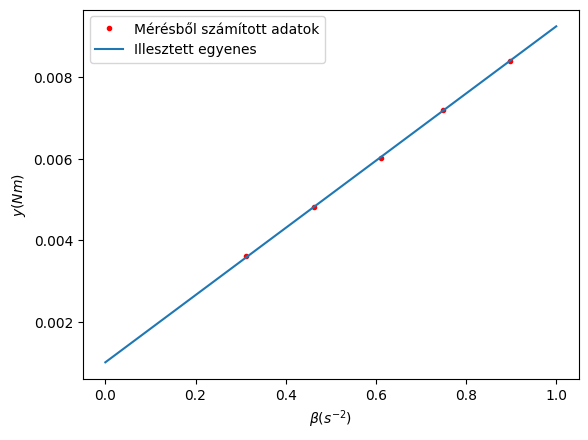
\includegraphics{./Henger_illesztes.png}
\end{figure}
%hibaszámítás, ábra
%%%%%%%%%%%%%%%%%%%%%%%%%%%%%%%%%%%%%%%%%%%%%%%%%%%%%%%%%%%%%%%%%%%%%%%%%%%%%%%%%%%%%%%%%%%%%%%%%%%%%%%%%%%%%%%%%%%%%%%%%%%%%%%%%%%%%%%%%%%%%%%%%%%%%%%%%%%%%%%%%%%%%%%%%%%%%%%
A rúd sugara $\rho=0.01005/2=0.005025m$, a fonáltárcsájának sugara pedig $r_{rud_tarcsa}$. Ebből $y$ és $\beta$ értékei:
\begin{table}[H]
    \centering
    \begin{tabular}{|r|r|r|}
        \hline
        Tömeg$(kg)$ & $y(Nm)$ & $\beta(s^{-2})$ \\
        \hline
        0.15 & 0.0038 & 1.634 \\
        \hline
        0.20 & 0.0050 & 2.157 \\
        \hline
        0.25 & 0.0062 & 2.706 \\
        \hline
        0.30 & 0.0075 & 3.294 \\
        \hline
        0.35 & 0.0087 & 3.830 \\
        \hline
    \end{tabular}
    \caption{$y$ és $\beta$ értékei a rúd esetében.}
\end{table}
A rúd esetében az $y$-ra kapott összefüggés a következő:
\begin{equation*}
    y=2.26\cdot 10^{-3}\beta+1.0\cdot 10^{-4}
\end{equation*}
Így $y_{ill}$ és $\Delta y$ értékei jelen esetben:
\begin{table}[H]
    \centering
    \begin{tabular}{|r|r|r|r|}
        $\beta(s^{-2})$ & $y(Nm)$ & $y_{ill}(Nm)$ & $\Delta y(Nm)$ \\
        \hline
        1.634 & 0.00375 & 0.00379 & -3.668$\cdot 10^{-5}$ \\
        \hline
        2.157 & 0.00500 & 0.00497 & 3.222$\cdot 10^{-5}$ \\
        \hline
        2.706 & 0.00624 & 0.00621 & 4.171$\cdot 10^{-5}$ \\
        \hline
        3.294 & 0.00749 & 0.00754 & -3.778$\cdot 10^{-5}$ \\
        \hline
        3.830 & 0.00875 & 0.00875 & 5.287$\cdot 10^{-7}$ \\
        \hline
    \end{tabular}
    \caption{$y$ és $y_{ill}$ összevetése a rúd esetében.}
\end{table}
Így a hibaszámítás a meredeksége:
\begin{equation*}
    \Delta \Theta_{rúd} = 2\frac{\left|\Delta y\right|_{max}}{\beta_{max}-\beta_{min}}=2*\frac{4.171\cdot 10^{-5}}{3.830-1.634}=3.8\cdot 10^{-5}
\end{equation*}
Ebből $\Theta_{rúd}=2.26\cdot 10^{-3}\pm3.8\cdot 10^{-5}kgm^2$.
Az illesztett egyenes és az adatpontok a következő ábrán láthatók:
\begin{figure}[H]
    \centering
    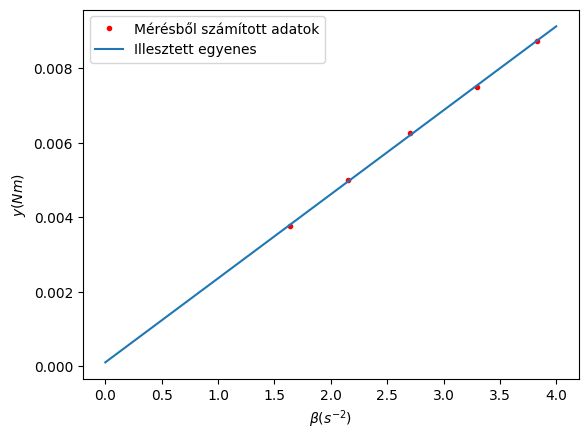
\includegraphics{./Rud_illesztes.png}
\end{figure}
%ábra
%%%%%%%%%%%%%%%%%%%%%%%%%%%%%%%%%%%%%%%%%%%%%%%%%%%%%%%%%%%%%%%%%%%%%%%%%%%%%%%%%%%%%%%%%%%%%%%%%%%%%%%%%%%%%%%%%%%%%%%%%%%%%%%%%%%%%%%%%%%%%%%%%%%%%%%%%%%%%%%%%%%%%%%%%%%%%%%
\subsection*{Tehetetlenségi nyomatékok számolása}
A korong esetében a tehetetlenségi nyomaték:
\begin{equation*}
    \Theta_{korong}=\frac{1}{2}mr_{korong}^2=\frac{1}{2}*1.511*0.10975^2=0,009100kgm^2
\end{equation*}
Ahol $\Theta_{korong}$ a korong tehetetlenségi nyomatéka, $m$ a korong tömege, $r_{korong}$ pedig a korong sugara.
Csak a tömeg hibáját vesszük figyelembe, amit a minta fonáltárca tömegének veszünk $\Delta m_{korong}=m_{tárcsa}=0.009kg$, a tehetetlenségi nyomaték hibáját hibaterjedéssel számíthatjuk ki: $\Delta\Theta_{korong}=\frac{1}{2}\Delta m_{korong}r_{korong}^2=\frac{1}{2}0.009*0.10975^2=5.4\cdot 10{-5}kgm^2$. \newline


A rúd esetében a tehetetlenségi nyomatékra vonatkozó képlet a következő:
\begin{equation*}
    \Theta_{rúd}=\frac{1}{12}mL^2+\frac{1}{4}m\rho^2=\frac{1}{12}*0.223*0.3590^2+\frac{1}{4}0.223*0.005025^2=0.002396kgm^2
\end{equation*}
Ahol $\rho$ a rúd sugara, $L$ a hossza, $m$ a tömege és $\Theta_{rúd}$ a tehetetlenségi nyomatéka.
Az előzőekez hasonlóan szintén csak a tömeg hibáját vesszük figyelembe, amely itt is $m_{tárcsa}=0.009kg$ lesz, tehát $\Delta \Theta_{rúd}=\Theta_{rúd}*\frac{\Delta m}{m}=9.7\cdot 10^{-5}kgm^2$.
\section*{Eredmények}
\begin{table}[H]
    \centering
    \begin{tabular}{|r|r|}
        \hline
        \multicolumn{2}{|c|}{Korong} \\
        \hline
        Mért tehetetlenségi nyomaték$(kgm^2)$ & $8.25\cdot 10^{-3}\pm{1.153\cdot 10^{-4}}$ \\
        \hline
        Számolt tehetetlenségi nyomaték$(kgm^2)$ & $9.10\cdot 10^{-3}\pm 5.4\cdot 10^{-5}$ \\
        \hline
    \end{tabular}
    \caption{A korong tehetetlenségi nyomatéka a két módszerrel.}
\end{table}
\begin{table}[H]
    \centering
    \begin{tabular}{|r|r|}
        \hline
        \multicolumn{2}{|c|}{Rúd} \\
        \hline
        Mért tehetetlenségi nyomaték$(kgm^2)$ & $2.26\cdot 10^{-3}\pm3.8\cdot 10^{-5}$ \\
        \hline
        Számolt tehetetlenségi nyomaték$(kgm^2)$ & $2.396\cdot 10^{-3}\pm9.7\cdot 10^{-5} $ \\
        \hline
    \end{tabular}
    \caption{A rúd tehetetlenségi nyomatéka a két módszerrel.}
\end{table}
\section*{Diszkusszió}
A két módszerrel kapott tehetetlenségi nyomatékok mindét test esetén jó közelíttéssel megegyeznek, ám nincsenek hibahatáron belül. Az eltérés nagyjából 5-10\% a két módszer eredménye között, amelyet okozhatnak az általunk elhanyagolt hibák, valamint az illesztési hiba számolásának módszere, és a hibaterjedési modellünk pontatlansága is beleszól a kapott eredménybe.
\end{document}

%rúd téglalap